% ============================================================
%  पिछला आवरण (Back cover) — मॉडर्न विज्ञान/तकनीक थीम
%  पुस्तक-परिचय · लेखक · QR · ISBN बारकोड · उद्धरण
% ============================================================
% ============================================================
%  cover-graphics.tex — साझा रंग, फ़ॉन्ट एवं TikZ चित्र
%  (आवरण front + back दोनों इसे \input करते हैं — guard ज़रूरी)
% ============================================================
\ifcsname cvGraphicsLoaded\endcsname\else
\expandafter\gdef\csname cvGraphicsLoaded\endcsname{}

% ---------------- बाल-सुलभ रंग-पट्टिका (playful palette - kept for compatibility) ----------------
\definecolor{cvSkyTop}{HTML}{63C7F2}
\definecolor{cvSkyBot}{HTML}{EAF8FF}
\definecolor{cvHill}{HTML}{7FC85A}
\definecolor{cvHillD}{HTML}{67B048}
\definecolor{cvBlue}{HTML}{1F4E79}
\definecolor{cvOrange}{HTML}{F5821F}
\definecolor{cvYellow}{HTML}{FFC83D}
\definecolor{cvRed}{HTML}{E5524A}
\definecolor{cvPurple}{HTML}{8E5BD9}
\definecolor{cvCyan}{HTML}{2FB4D6}
\definecolor{cvPink}{HTML}{FF7BAC}
\definecolor{cvLime}{HTML}{9CD356}
\definecolor{cvGrey}{HTML}{5F6368}

% ---------------- मॉडर्न विज्ञान/तकनीक रंग-पट्टिका (Modern Tech Palette) ----------------
\definecolor{cvBgDark}{HTML}{080D1A}
\definecolor{cvBgMid}{HTML}{0E1830}
\definecolor{cvBgLight}{HTML}{1A2B4C}
\definecolor{cvNeonCyan}{HTML}{00F2FE}
\definecolor{cvNeonBlue}{HTML}{4FACFE}
\definecolor{cvNeonPurple}{HTML}{E255FF}
\definecolor{cvNeonPink}{HTML}{FF0844}
\definecolor{cvNeonGreen}{HTML}{38EF7D}
\definecolor{cvNeonYellow}{HTML}{F9D423}
\definecolor{cvNeonOrange}{HTML}{FF5E62}
\definecolor{cvGridColor}{HTML}{14244A}

% ---------------- फ़ॉन्ट (Baloo 2 — rounded, Devanagari + Latin) ----------------
% ucharclasses को स्थानीय रूप से बंद कर (\XeTeXinterchartokenstate=0) एक ही
% फ़ॉन्ट से दोनों लिपियाँ — एकरूप, मज़ेदार शैली।
% Devanagari shaping needs Script=Devanagari; Latin uses default. अलग families।
\newfontfamily\cvTitleDev{Baloo2-ExtraBold.ttf}[Path=fonts/, Script=Devanagari, Language=Hindi]
\newfontfamily\cvHeadDev{Baloo2-SemiBold.ttf}[Path=fonts/, Script=Devanagari, Language=Hindi]
\newfontfamily\cvBodyDev{Baloo2-Medium.ttf}[Path=fonts/, Script=Devanagari, Language=Hindi]
\newfontfamily\cvTitleLat{Baloo2-ExtraBold.ttf}[Path=fonts/]
\newfontfamily\cvHeadLat{Baloo2-SemiBold.ttf}[Path=fonts/]
\newfontfamily\cvBodyLat{Baloo2-Medium.ttf}[Path=fonts/]
% \cvXX : ucharclasses बंद कर Baloo चुनें — H=हिन्दी, L=Latin
\newcommand{\cvTH}{\XeTeXinterchartokenstate=0 \cvTitleDev}
\newcommand{\cvTL}{\XeTeXinterchartokenstate=0 \cvTitleLat}
\newcommand{\cvHH}{\XeTeXinterchartokenstate=0 \cvHeadDev}
\newcommand{\cvHL}{\XeTeXinterchartokenstate=0 \cvHeadLat}
\newcommand{\cvBH}{\XeTeXinterchartokenstate=0 \cvBodyDev}
\newcommand{\cvBL}{\XeTeXinterchartokenstate=0 \cvBodyLat}

% ---------------- चित्र (pics) ----------------
\tikzset{
  planet/.pic={
    \draw[cvNeonPurple, line width=2pt] (0,0) ellipse (1.15 and 0.42);
    \fill[cvNeonOrange] (0,0) circle (0.7);
    \fill[cvNeonOrange!70] (0.22,0.18) circle (0.18);
    \fill[cvNeonOrange!70!black] (-0.25,-0.12) circle (0.12);
    \draw[cvNeonPurple, line width=2pt] (1.15,0) arc (0:180:1.15 and 0.42);
  },
  rocket/.pic={
    \fill[cvNeonOrange] (0,-0.95) -- (-0.2,-0.5) -- (0,-0.64) -- (0.2,-0.5) -- cycle;
    \fill[cvNeonYellow] (0,-0.8) -- (-0.1,-0.5) -- (0,-0.6) -- (0.1,-0.5) -- cycle;
    \fill[cvNeonPink] (-0.3,-0.5) -- (-0.56,-0.78) -- (-0.3,-0.18) -- cycle;
    \fill[cvNeonPink] (0.3,-0.5) -- (0.56,-0.78) -- (0.3,-0.18) -- cycle;
    \fill[white] (-0.3,-0.5) .. controls (-0.32,0.45) .. (0,1.0)
                 .. controls (0.32,0.45) .. (0.3,-0.5) -- cycle;
    \draw[cvNeonBlue, line width=1.5pt] (-0.3,-0.5) .. controls (-0.32,0.45) .. (0,1.0)
                 .. controls (0.32,0.45) .. (0.3,-0.5) -- cycle;
    \fill[cvNeonPink] (0,1.0) .. controls (0.18,0.55) .. (0.15,0.35) -- (-0.15,0.35)
                 .. controls (-0.18,0.55) .. cycle;
    \fill[cvNeonCyan] (0,0.05) circle (0.15);
    \draw[cvNeonBlue, line width=1pt] (0,0.05) circle (0.15);
  },
  atom/.pic={
    \draw[cvNeonCyan, line width=1.4pt] (0,0) ellipse (0.95 and 0.36);
    \draw[cvNeonCyan, line width=1.4pt, rotate=60] (0,0) ellipse (0.95 and 0.36);
    \draw[cvNeonCyan, line width=1.4pt, rotate=-60] (0,0) ellipse (0.95 and 0.36);
    \fill[cvNeonPink] (0,0) circle (0.17);
    \fill[cvNeonBlue] (0.95,0) circle (0.08);
    \fill[cvNeonBlue] (-0.48,0.82) circle (0.08);
    \fill[cvNeonBlue] (-0.48,-0.82) circle (0.08);
  },
  dna/.pic={
    \draw[cvNeonPink, line width=1.8pt] plot[domain=0:360, samples=46] ({0.32*sin(\x)},{\x/130 - 1.38});
    \draw[cvNeonPurple, line width=1.8pt] plot[domain=0:360, samples=46] ({-0.32*sin(\x)},{\x/130 - 1.38});
    \foreach \t in {25,65,...,335}
      \draw[cvNeonCyan, line width=1pt] ({0.32*sin(\t)},{\t/130 - 1.38}) -- ({-0.32*sin(\t)},{\t/130 - 1.38});
  },
  flask/.pic={
    \fill[cvNeonCyan!20] (-0.1,0.6) -- (-0.1,0.16) -- (-0.45,-0.5) -- (0.45,-0.5) -- (0.1,0.16) -- (0.1,0.6) -- cycle;
    \fill[cvNeonGreen] (-0.3,-0.15) -- (-0.45,-0.5) -- (0.45,-0.5) -- (0.3,-0.15) -- cycle;
    \draw[cvNeonBlue, line width=1.3pt] (-0.1,0.6) -- (-0.1,0.16) -- (-0.45,-0.5) -- (0.45,-0.5) -- (0.1,0.16) -- (0.1,0.6);
    \draw[cvNeonBlue, line width=1.3pt] (-0.17,0.6) -- (0.17,0.6);
    \fill[white] (0.07,-0.3) circle (0.045);
    \fill[white] (-0.12,-0.38) circle (0.03);
  },
  bulb/.pic={
    \fill[cvNeonYellow] (0,0) circle (0.33);
    \draw[cvNeonOrange, line width=1pt] (0,0) circle (0.33);
    \fill[cvGrey!55] (-0.14,-0.3) rectangle (0.14,-0.46);
    \draw[cvNeonOrange, line width=1pt] (-0.08,0.12) -- (0,-0.04) -- (0.08,0.12);
    \foreach \a in {45,90,135} \draw[cvNeonYellow, line width=1.4pt] (\a:0.42) -- (\a:0.58);
  },
  robot/.pic={
    \draw[cvGrey, line width=2.4pt] (0,1.0) -- (0,1.35);
    \fill[cvRed] (0,1.45) circle (0.12);
    \fill[white] (-1,-0.85) rectangle (1,1.0);
    \draw[cvBlue, line width=2.4pt, rounded corners=10pt] (-1,-0.85) rectangle (1,1.0);
    \fill[cvRed, rounded corners=2pt] (-1.2,0.0) rectangle (-1.0,0.45);
    \fill[cvRed, rounded corners=2pt] (1.0,0.0) rectangle (1.2,0.45);
    \fill[cvBlue!88, rounded corners=8pt] (-0.8,-0.58) rectangle (0.8,0.78);
    \fill[cvCyan] (-0.4,0.26) circle (0.17);
    \fill[cvCyan] (0.4,0.26) circle (0.17);
    \fill[white] (-0.34,0.33) circle (0.06);
    \fill[white] (0.46,0.33) circle (0.06);
    \draw[cvYellow, line width=2.2pt] (-0.32,-0.22) .. controls (0,-0.46) .. (0.32,-0.22);
  },
  cyber_robot/.pic={
    % shoulders
    \fill[white!92!cvBgMid, rounded corners=6pt] (-0.7,-0.6) -- (-0.8,-0.2) -- (0.8,-0.2) -- (0.7,-0.6) -- cycle;
    \draw[cvNeonCyan, line width=1.5pt] (-0.7,-0.6) -- (-0.8,-0.2) -- (0.8,-0.2) -- (0.7,-0.6) -- cycle;
    % neck
    \fill[cvBgLight] (-0.2,-0.2) rectangle (0.2,0.0);
    \draw[cvNeonCyan, line width=1pt] (-0.2,-0.2) -- (-0.2,0.0) (0.2,-0.2) -- (0.2,0.0);
    % head
    \fill[white, rounded corners=12pt] (-0.6,0.0) rectangle (0.6,0.9);
    \draw[cvNeonBlue, line width=1.8pt, rounded corners=12pt] (-0.6,0.0) rectangle (0.6,0.9);
    % visor/eyes (glowing)
    \fill[cvBgDark, rounded corners=6pt] (-0.45,0.2) rectangle (0.45,0.6);
    \draw[cvNeonCyan, line width=1.2pt, rounded corners=6pt] (-0.45,0.2) rectangle (0.45,0.6);
    \fill[cvNeonCyan] (-0.22,0.4) circle (0.06);
    \fill[cvNeonCyan] (0.22,0.4) circle (0.06);
    \draw[cvNeonCyan, opacity=0.4, line width=1.5pt] (-0.35,0.4) -- (0.35,0.4);
    % antenna
    \draw[cvNeonBlue, line width=2pt] (0,0.9) -- (0,1.25);
    \fill[cvNeonPurple] (0,1.3) circle (0.1);
    \fill[cvNeonPurple, opacity=0.3] (0,1.3) circle (0.22);
  },
  chip/.pic={
    \foreach \x in {-0.32,0,0.32}{
      \fill[cvGrey] (\x,0.55) rectangle ++(0.1,0.14);
      \fill[cvGrey] (\x,-0.69) rectangle ++(0.1,0.14);
    }
    \foreach \y in {-0.32,0,0.32}{
      \fill[cvGrey] (0.55,\y) rectangle ++(0.14,0.1);
      \fill[cvGrey] (-0.69,\y) rectangle ++(0.14,0.1);
    }
    \fill[cvNeonOrange, rounded corners=5pt] (-0.58,-0.58) rectangle (0.58,0.58);
    \node[white, font=\cvHeadLat] at (0,0) {AI};
  },
}

% ---- सहायक मैक्रो: तारा एवं चमक (star & sparkle) ----
\newcommand{\cvstar}[3]{%
  \node[star, star points=5, star point ratio=0.46, fill=#3, scale=#2, inner sep=0pt] at (#1) {};
}
\newcommand{\cvsparkle}[3]{%
  \node[star, star points=4, star point ratio=0.28, fill=#3, scale=#2, inner sep=0pt] at (#1) {};
}

\fi

\clearpage
\thispagestyle{empty}

% Force page generation so the overlay renders on a clean blank page
\mbox{}

\begin{tikzpicture}[remember picture, overlay]
  % ---------- पृष्ठभूमि (dark space gradient matching front cover) ----------
  \shade[top color=cvBgDark, bottom color=cvBgMid]
        (current page.south west) rectangle (current page.north east);
  
  % Subtle grid pattern
  \draw[step=1.2cm, cvGridColor, line width=0.4pt, opacity=0.45] 
        (current page.south west) grid (current page.north east);

  % Subtle flowing data pathways in the background (symmetrical to front cover)
  \draw[cvNeonCyan, opacity=0.15, line width=1.5pt] (-10.5, 6.0) .. controls (-3.0, 4.0) and (3.0, -8.0) .. (10.5, -6.0);
  \draw[cvNeonPurple, opacity=0.12, line width=1.2pt] (-10.5, -4.0) .. controls (-4.0, 2.0) and (4.0, 8.0) .. (10.5, 4.0);

  \coordinate (C) at (current page.center);

  % ---------------- 1. पुस्तक परिचय (Top Card) ----------------
  % Glassmorphism style card body (semi-transparent dark backdrop with neon border)
  \filldraw[fill=cvBgLight!35!cvBgDark, draw=cvNeonCyan, line width=1.5pt, rounded corners=15pt] 
           ($(C)+(-8.5, 4.3)$) rectangle ($(C)+(8.5, 10.3)$);
           
  % Title banner
  \node[fill=cvBgLight!80!cvBgDark, rounded corners=12pt, draw=cvNeonCyan, line width=1.2pt, 
        text=white, font=\cvHH\fontsize{16}{20}\selectfont, 
        inner xsep=22pt, inner ysep=7pt] 
        at ($(C)+(0, 10.3)$) {पुस्तक परिचय};
        
  % Text inside card (white text for maximum contrast on dark mode)
  \node[text width=13.0cm, align=justify, text=white, font=\cvBH\fontsize{10.5}{14.5}\selectfont] 
        at ($(C)+(0, 7.1)$) {%
    कृत्रिम बुद्धिमत्ता (Artificial Intelligence) आधुनिक विज्ञान की सबसे क्रांतिकारी
    तकनीकों में से एक है। यह पुस्तक विद्यार्थियों को AI की मूलभूत अवधारणाओं, मशीन लर्निंग,
    data विश्लेषण, वैज्ञानिक अनुसंधान, स्वास्थ्य विज्ञान, अंतरिक्ष अन्वेषण, पर्यावरण अध्ययन
    तथा भविष्य की उभरती प्रौद्योगिकियों से परिचित कराती है।\par\medskip
    सरल भाषा, वास्तविक उदाहरणों और रोचक चित्रों के माध्यम से यह पुस्तक विज्ञान और AI के
    अद्भुत संगम को समझने का एक प्रभावी माध्यम है। यह विद्यार्थियों में वैज्ञानिक सोच, नवाचार
    और भविष्य की तकनीकों के प्रति जिज्ञासा विकसित करने के उद्देश्य से तैयार की गई है।
  };
  
  % Overlapping science icons (Canva style, neon themes)
  \pic[scale=1.1] at ($(C)+(-8.3, 7.8)$) {dna};
  \pic[scale=0.7] at ($(C)+(-8.5, 5.0)$) {atom};
  \pic[scale=0.8] at ($(C)+(8.3, 8.8)$) {planet};
  \pic[scale=0.95] at ($(C)+(8.2, 5.0)$) {flask};


  % ---------------- 2. लेखक परिचय (Middle Card) ----------------
  % Glassmorphism card body (glowing neon-blue outline)
  \filldraw[fill=cvBgLight!35!cvBgDark, draw=cvNeonBlue, line width=1.5pt, rounded corners=15pt] 
           ($(C)+(-8.5, -2.3)$) rectangle ($(C)+(8.5, 2.7)$);
           
  % Title banner
  \node[fill=cvBgLight!80!cvBgDark, rounded corners=12pt, draw=cvNeonBlue, line width=1.2pt, 
        text=white, font=\cvHH\fontsize{16}{20}\selectfont, 
        inner xsep=22pt, inner ysep=7pt] 
        at ($(C)+(0, 2.7)$) {लेखक परिचय};
        
  % Circular photo of the author with neon cyan glow outline
  \begin{scope}
    \clip ($(C)+(-5.8, 0.1)$) circle (1.25);
    \node at ($(C)+(-5.8, 0.1)$) {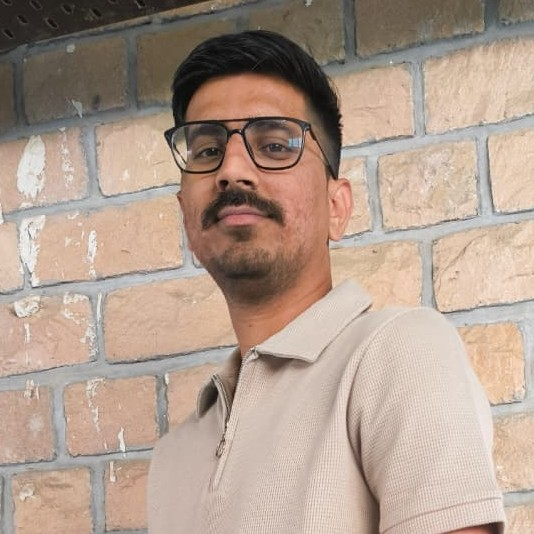
\includegraphics[width=2.5cm]{images/author.jpg}};
  \end{scope}
  \draw[cvNeonCyan, line width=2.0pt] ($(C)+(-5.8, 0.1)$) circle (1.25);
  
  % Author details (glowing white / neon cyan)
  \node[anchor=west, text=cvNeonCyan, font=\cvHH\fontsize{16}{20}\selectfont] 
        at ($(C)+(-4.2, 1.4)$) {कृष्ण कुमार गोदारा};
        
  \node[anchor=north west, text width=10.4cm, align=justify, text=white, font=\cvBH\fontsize{9.5}{13.5}\selectfont] 
        at ($(C)+(-4.3, 1.0)$) {%
    भारतीय प्रौद्योगिकी संस्थान (IIT) जोधपुर में भौतिकी विभाग के अंतर्गत PhD शोधार्थी (JRF)
    हैं। उनका शोध कार्य सक्रिय पदार्थ (Active Matter), गैर-संतुलन प्रणालियों तथा कम्प्यूटेशनल
    भौतिकी पर केंद्रित है।\par\smallskip
    उन्होंने \textbf{CSIR-UGC NET-JRF 2024 (भौतिक विज्ञान)} में अखिल भारतीय रैंक \textbf{46}
    प्राप्त की। उनका उद्देश्य आधुनिक विज्ञान, कृत्रिम बुद्धिमत्ता और कम्प्यूटेशनल तकनीकों को
    विद्यार्थियों तक सरल एवं प्रेरणादायक रूप में पहुँचाना है।
  };


  % ---------------- 3. संपर्क सूत्र (QR Codes) ----------------
  \node[draw=cvNeonCyan, line width=1.2pt, fill=white, inner sep=1.5pt, rounded corners=2pt] 
        (linkedin) at ($(C)+(-4.5, -4.5)$) {
\includegraphics[width=2.1cm]{images/Linkedin.png}};
  \node[draw=cvNeonCyan, line width=1.2pt, fill=white, inner sep=1.5pt, rounded corners=2pt] 
        (instagram) at ($(C)+(0, -4.5)$) {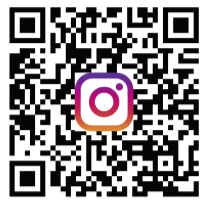
\includegraphics[width=2.1cm]{images/Instagram.png}};
  \node[draw=cvNeonCyan, line width=1.2pt, fill=white, inner sep=1.5pt, rounded corners=2pt] 
        (github) at ($(C)+(4.5, -4.5)$) {
\includegraphics[width=2.1cm]{images/github.png}};


  % ---------------- 4. उद्धरण एवं चित्र (Bottom Quote Card) ----------------
  % AI Core (Left)
  \fill[cvBgDark, draw=cvNeonCyan, line width=2pt] ($(C)+(-6.8, -9.2)$) circle (1.1);
  \pic[scale=1.3] at ($(C)+(-6.8, -9.2)$) {chip};
  
  % Speech bubble/rounded card for quote (neon purple frame)
  \filldraw[fill=cvBgLight!35!cvBgDark, draw=cvNeonPurple, line width=1.5pt, rounded corners=12pt] 
           ($(C)+(-4.5, -10.8)$) rectangle ($(C)+(7.2, -7.6)$);
           
  % Quote Text (white/neon orange)
  \node[text width=11.0cm, align=center, text=white, font=\cvHH\fontsize{14}{20}\selectfont] 
        at ($(C)+(1.35, -9.2)$) {%
    \color{white} “आज की जिज्ञासा, कल की खोज बनती है;\\
    और {\color{cvNeonOrange}कृत्रिम बुद्धिमत्ता} उस खोज को नई दिशा देती है।”
  };
  
  % Graphics on the right
  \pic[scale=0.8, rotate=30] at ($(C)+(8.4, -9.5)$) {rocket};
  \pic[scale=0.5] at ($(C)+(6.8, -7.5)$) {atom};


  % ---------------- 5. संस्करण एवं बारकोड (Bottom-most details) ----------------
  % Left edition text
  \node[anchor=west, text=cvNeonCyan, font=\cvHH\fontsize{9.5}{12}\selectfont] 
        at ($(C)+(-8.5, -13.2)$) {
    प्रथम संस्करण (First Edition) ~$\cdot$~ 2026\\[2pt]
    \color{white!80} स्वप्रकाशित (Self-published)
  };
  
  % Right barcode (white container with neon border)
  \node[anchor=east] at ($(C)+(8.5, -12.8)$) {
    \fcolorbox{cvNeonCyan}{white}{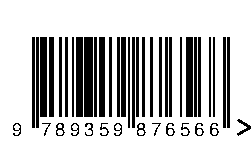
\includegraphics[height=1.5cm]{images/isbn-barcode.pdf}}
  };
  \node[anchor=east, text=white, font=\cvHH\fontsize{8.5}{10}\selectfont] 
        at ($(C)+(8.5, -13.9)$) {ISBN 978-93-5987-656-6};

\end{tikzpicture}
\clearpage
